\addcontentsline{toc}{section}{Введение}
\chapter{Введение}
\justify
Проблема поиска пересечений линий на изображении является очень распространенной и её решение может быть использовано в таких задачах компьютерного зрения как:
\begin{enumerate}
	\item Автоматическое определение полей во время спортивных трансляций
	\item Детектирование ориентиров при автоматическом управлении роботом
	\item Детектирование железнодорожных стрелок на изображении, сделанном с локомотива поезда
\end{enumerate} 


В данной работе будут рассмотрены подходы к решению задачи применительно к детектированию ж/д стрелок.


Для автоматизации процесса управления поездом необходимо создать систему, которая позволяла бы стать надежным автоматическим ассистентом/помощником для машиниста локомотива (стать неким driving assistance), но ни в коем случае не заменить действия человека полностью. 
Одной из задач такой системы является обнаружение железнодорожных стрелок для обеспечения движения поезда по правильному пути.
Решение этой задачи позволит обнаруживать разветвления пути заранее (визуально) и анализировать возможные дальнейшие пути движения поезда, выдавая полезную информацию для машиниста локомотива, такую как: "на правой ветке обнаружены вагоны - путь занят!". Это решение значительно повысит безопасность движения на железных дорогах.

\newpage
\section{Постановка задачи}
На вход подается изображение — фотография сделанная с головы поезда. Необходимо найти на входном изображении места пересечений железно-дорожных путей. Пересечением будем называть точку, в которой пересекаются рельсы одной ж/д колеи с другой. На выходе алгоритма должен быть набор точек, в которых было обнаружено пересечение.

\begin{figure}[!h]
	\centering
	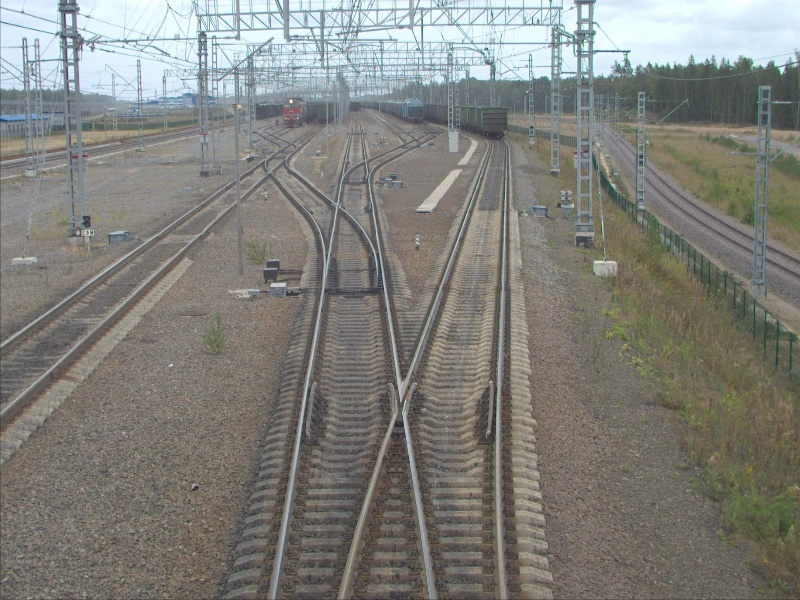
\includegraphics[width=0.9\textwidth]{pictures/img0002.jpg} 
	\caption{Пример входного изображения}
	\label{fig:input}
\end{figure}

\newpage
Замечания: 
\begin{enumerate}
	\item Точность поиска стрелок - окрестность от 20x20 до 50x50 пикселей(в зависимости от дальности стрелки)
	\item Необходимо правильно находить стрелки в пределах 20-30 метрах перед поездом. Нет задачи детектировать стрелки, которые находятся слишком далеко от поезда(40 метров и далее).
\end{enumerate}

\section{Обзор литературы}
Существует несколько глобальных подходов к поиску объектов на изображении:
\begin{enumerate}
	\item Сопоставление границ, градиентов и чёрно-белых пикселей изображения. Этот подход устойчив к изменению света, но не устойчив к изменению положения объекта на изображении(вращение, угол наклона).\cite{b:edge_match}.
	\item Поиск объекта по геометрическим свойствам. Если форма искомого объекта может быть задача аналитически, то такие объекты можно искать с помощью преобразования Хафа \cite{b:hough_transform}.
	\item Подход, основанный на сопоставлении признаков ключевых точек изображения с ключевыми точками искомого объекта. Данный подход реализован в следующих методах: SIFT\cite{b:SIFT}, SURF\cite{b:SURF}.
	\item Обучение классификатора на размеченных данных. В роли классификатора может быть: SVM классификатор\cite{b:SVM}, дерево решений \cite{b:decision_tree}, KNN классификатор \cite{b:knn}. В качестве входных векторов для классификаторов могут быть использованы различные виды признаков, полученные из размеченных изображений. 
	Например, гистограмма ориентированных градиентов(HOG)\cite{b:HOG},
	SURF\cite{b:SIFT}/SIFT\cite{b:SURF} дескрипторы и так далее. 
	
\end{enumerate}
Рассмотрим данные подходы подробнее.
\subsection{Поиск объекта по его геометрическим свойствам}
Для поиска объектов, геометрическая форма которых может быть задана некоторым уравнением(н-р прямая, круг, эллипс) используется следующий подход:
\begin{enumerate}
	\item Из изображения извлекаются границы. Это можно сделать с помощью алгоритма Canny \cite{b:canny}. \newline
	Пример применения алгоритма Canny к входному изображению:
	\begin{figure}[!h]
		\centering
		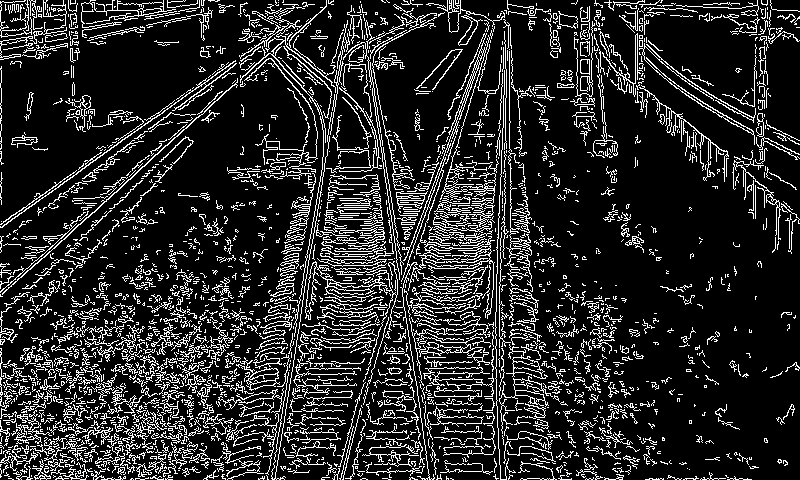
\includegraphics[width=0.9\textwidth]{pictures/canny_res}
		\caption[Применение алгоритма Canny]{}
		\label{fig:cannyres}
	\end{figure}
	\item После чего к полученным границам применяется алгоритма Хафа \ref{hough}. Если целью является поиск прямых, то алгоритм Хафа даст следующий результат(красным обозначены найденные линии):
	\begin{figure}[!h]
		\centering
		\begin{minipage}{0.45\textwidth}
			\centering
			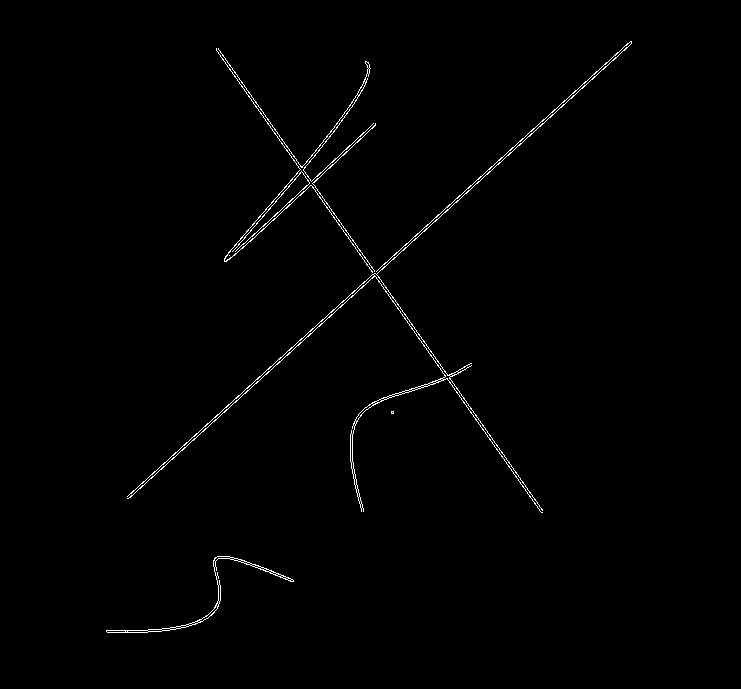
\includegraphics[width=0.7\linewidth]{pictures/canny_ex}
			\caption[Y]{}
			\label{fig:canny_ex}
		\end{minipage}
		\begin{minipage}{0.45\textwidth}
			\centering
			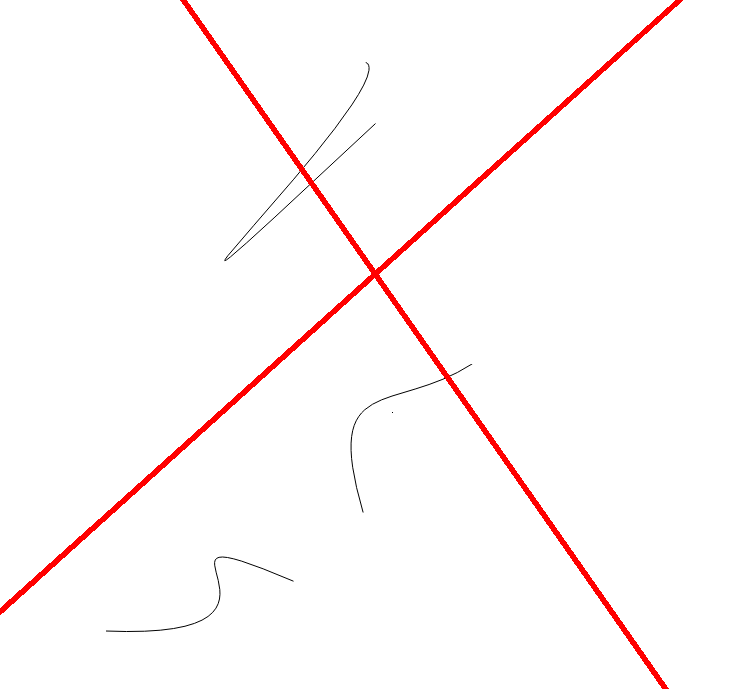
\includegraphics[width=0.7\linewidth]{pictures/hough_ex}
			\caption[X]{}
			\label{fig:hough_ex}
		\end{minipage}
	\end{figure}
\end{enumerate}

Таким образом, если требуется искать пересечения прямых линий на изображении, то для этого отлично подойдет следующий алгоритм:
\begin{enumerate}
	\item Поиск границ \cite{b:canny}
	\item Поиск линий \ref{hough}
	\item Поиск пересечений линий, найденных в предыдущем шаге. Это можно сделать аналитически. Для каждой пары найденных прямых составляем систему уравнений, тогда если эти прямые не параллельны, то решением системы будет точка пересечения прямых.
	$
	\begin{cases}
	a_1x + b_1y = c_1 
	\\
	a_2x + b_2y = c_2 
	\end{cases}
	$
\end{enumerate}

\paragraph{Предыдущие работы, посвященные поиску ж/д путей и их пересечений с помощью применения геометрически ориентированного подхода}

\subparagraph{Vision based rail track and switch recognition for self-localization of trains in a rail network \cite{b:hough_work1}.}

Подход, описанный в данной работе основан на анализе изображения с камеры, стоящей в голове
поезда. Условиями для корректного определения стрелок на железной дороге является то, что
расстояние между параллельными рельсами всегда одинаковое, а также радиус кривизны рельсов
достаточно большой.

В данной работе съёмка ж/д путей происходит достаточно часто, и к каждому вновь сделанному снимку применяется следующий алгоритм:

1. Из изображения вырезается близкая к поезду полоса.
\begin{figure}[!h]
	\centering
	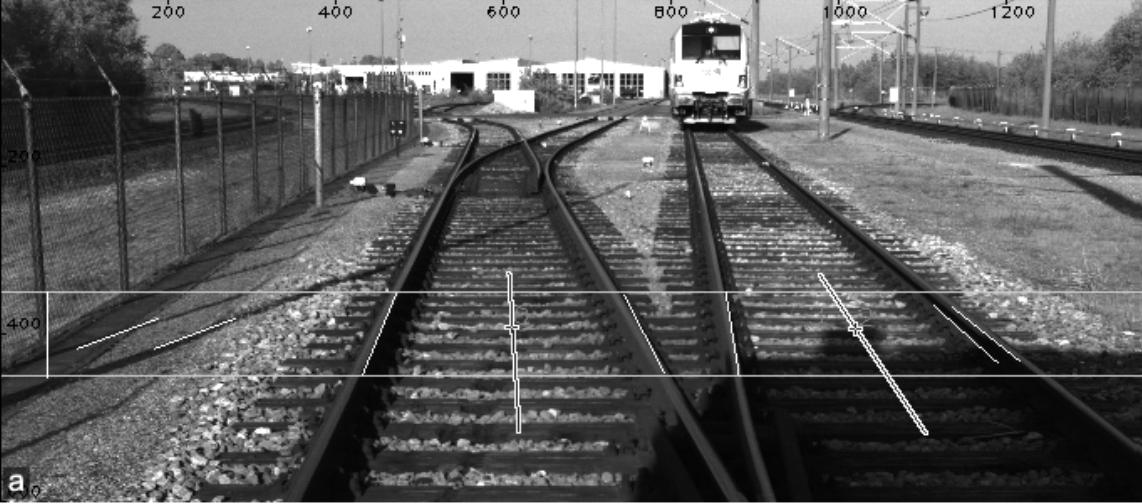
\includegraphics[width=0.9\linewidth]{pictures/screenshot001}
	\caption{}
	\label{fig:screenshot001}
\end{figure}

2. К выделенному участку применяется алгоритм поиска ребер: 
\begin{enumerate}
	\item Рассчитывается вектор градиента в каждой точке изображения
	\item Далее рассматриваются окрестности по 3x3 пикселя. И для каждого пикселя с величиной градиента большей, чем у половины соседей в окрестности выполняется следующая
	процедура: 
	Строится матрица ковариаций данного пикселя с соседями в окрестности 3х3. 
	$
	S = \left(
	\begin{array}{cccc}
	Cov_{xx} & Cov_{xy}\\
	Cov_{yx} & Cov_{yy}\\
	\end{array}
	\right), где
	Cov_{ab} = \dfrac{1}{n} \sum_{1}^{N} (g_a, g_b)
	$ 
	\item Вычисляются собственные числа этой матрицы, и если выполнены неравенства:
	$
	\begin{cases}
	\lambda_1 \geq t_l\\
	\dfrac{\lambda_2}{\lambda_1} \geq m_l 
	\end{cases}
	$
	,где $t_l, m_l$ вычисленные эмперическим путём константы, то данный пиксель считается
	краевым.
	Также из матрицы ковариации получаются два собственных вектора:
	$e_1, e_2$, больший из которые перпендикулярен краю, а меньший параллелен краю в данной точке.
\end{enumerate}
В итоге границы найденные границы выделенного блока выглядят следующим образом:
\begin{figure}[!h]
	\centering
	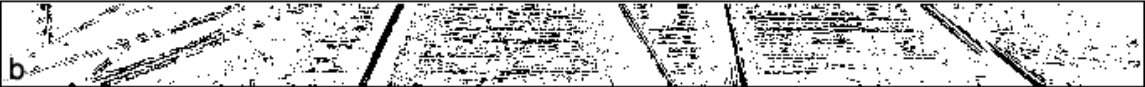
\includegraphics[width=0.9\linewidth]{pictures/screenshot002}
	\caption{}
	\label{fig:screenshot002}
\end{figure}

3. Поиск прямых.

Строится массив аккумулятор$A(\theta, x)$(по аналогии с алгоритмом Хафа\cite{b:hough_transform}). И для каждого краевого пикселя(K) вычисляется угол $\theta$ между большим собственным вектором $e_2$ и осью OY. 
Также необходимо вычислить значение $x_c$. Строится дополнительная прямая $y_c$ = $\dfrac{H}{2}$, где H - высота рассматриваемого изображения. Тогда $x_c$ будет координатой $x$ точки пересечения построенной прямой $y_c$ и продолжения собственного вектора $e_2$.
Увеличиваем значения аккумулятора $A(\theta, x_c)$ = $A(\theta, x_c) + 1$.
В итоге максимумы аккумулятора будут соответствовать параметрам прямых линий на изображении. На рисунке найденные линии обозначены черными точками.
\begin{figure}[!h]
	\centering
	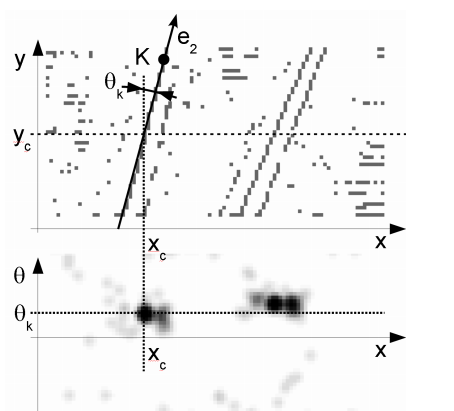
\includegraphics[width=0.9\linewidth]{pictures/screenshot004}
	\caption{}
	\label{fig:screenshot004}
\end{figure}
\newpage
Данный алгоритм работает значительно быстрее преобразования Хафа(ускорение достигается за счет сохранения времени, которое в алгоритме Хафа тратится на перебор $\theta \in [0, \pi]$).
При этом алгоритм качественно находит прямые линии, проходящие через центральную вертикальную ось изображения.

4. Выделение ж/д колеи по найденным прямым.

В данном алгоритме предполагается, что ширина железнодорожной колеи заранее зафиксирована и приходит на вход алгоритму. 

Поэтому чтобы найти пары рельсов, принадлежащих к одной колее нужно выполнить перебор по всем найденным рельсам, сравнивая при этом расстояние между ними с эталонным расстоянием между рельсами(с некоторой погрешностью $\delta R$).

Но нельзя забывать про то, что изображение делается с камеры и нужно учитывать перспективную проекцию \cite{b:projection} точек изображения на точки в реальном мире, чтобы корректно сравнивать расстояние между рельсами на изображении с расстоянием в мировой системе координат.
В итоге результат поиска ж/д колеи следующий(на рисунке выделен горизонтальный блок и линии, соответствующие центрам найденных пар рельсов):
\begin{figure}[!h]
	\centering
	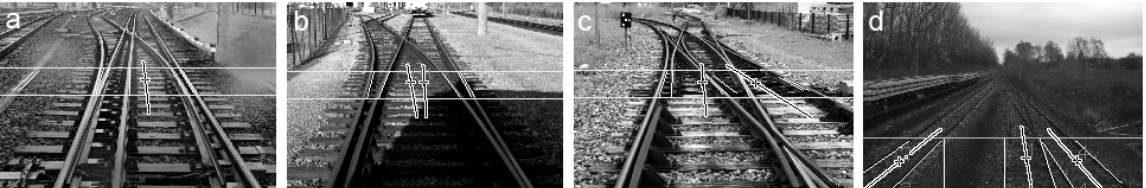
\includegraphics[width=1\linewidth,height=0.5\linewidth]{pictures/screenshot006}
	\caption{}
	\label{fig:screenshot006}
\end{figure}

5. Определение стрелок.

При поиске пересечений найденных рельсов учтем, что нам известен минимальный радиус
кривой, по которой может двигаться поезд(является параметром алгоритма). Из данного радиуса можно вычислить максимальное боковое отклонение $s_1$, на которое должен отклониться центр колеи, чтобы считаться НЕ основной колеёй. 

Таким образом, мы ожидаем, что одна из наблюдаемых нами колея всегда имеет боковое отклонение от центра поезда принадлежащее интервалу [$-s_1$, $s_1$].
Если центр колеи становится < $-s_1$, то это означается, что данная колея является левой веткой основной колеи, в обратном случае правой веткой. В момент времени, когда
происходит переход данной границы мы можем отметить, что поезд прошел стрелку.
\newpage
На рисунке обозначены границы $s_1$(теоретическая граница) и $s_2$(экспериментальная граница), где $s_2$ = $s_1$ + $\delta s$(подобрана экспериментально). Пересечение фиксируется в момент времени, когда центр колеи переходит границу $|s_2|$(это место показано стрелками на рисунке).
\begin{figure}[!h]
	\centering
	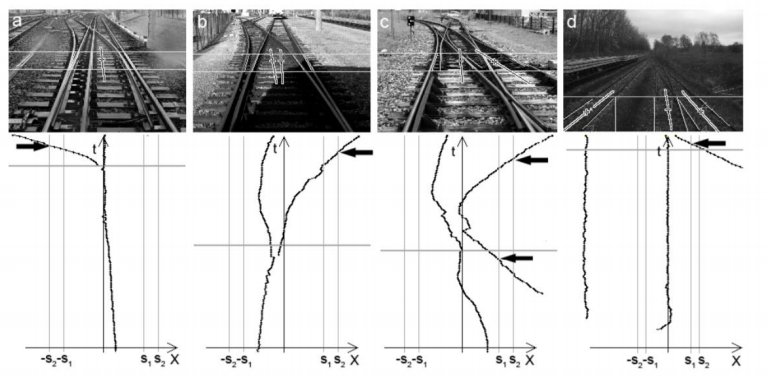
\includegraphics[width=1\linewidth]{pictures/screenshot008}
	\caption{}
	\label{fig:screenshot008}
\end{figure}

На левом рисунке видно, что есть отклоняющаяся налево колея и поезда пойдет прямо.
На втором слева рисунке видно, что линия соответствующая прямой колее отклоняется вправо, следовательно поезд прошёл по левой колее и т.д.

\subparagraph{Efficient railway tracks detection and turnouts recognition method using HOG features \cite{b:growing_up}}.

В данном работе описывается метод поиска железнодорожных путей с использованием Histogram of oriented gradients\cite{b:HOG}(гистограмма ориентированных градиентов).

\newpage
Алгоритм следующий:

1. Входное изображение разбивается на сетку, с уменьшением размера блока в зависимости от координаты Y на изображении(это сделано чтобы имитировать перспективную проекцию).
\begin{figure}[!h]
	\centering
	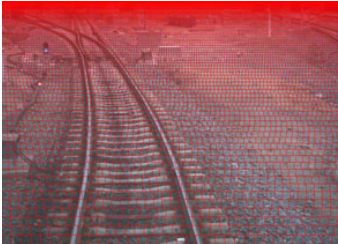
\includegraphics[width=1\linewidth]{pictures/screenshot009}
	\caption{}
	\label{fig:screenshot009}
\end{figure}

2. Начиная с нижней строки сетки применяется алгоритм growing up, который на основе похожести HOG соседних верхних клеток расширяет множество схожих кусочкой изображения.
В итоге на выходе алгоритма growing up имеем множество рельсов(на рисунке обозначены разными цветами).
\begin{figure}[!h]
	\centering
	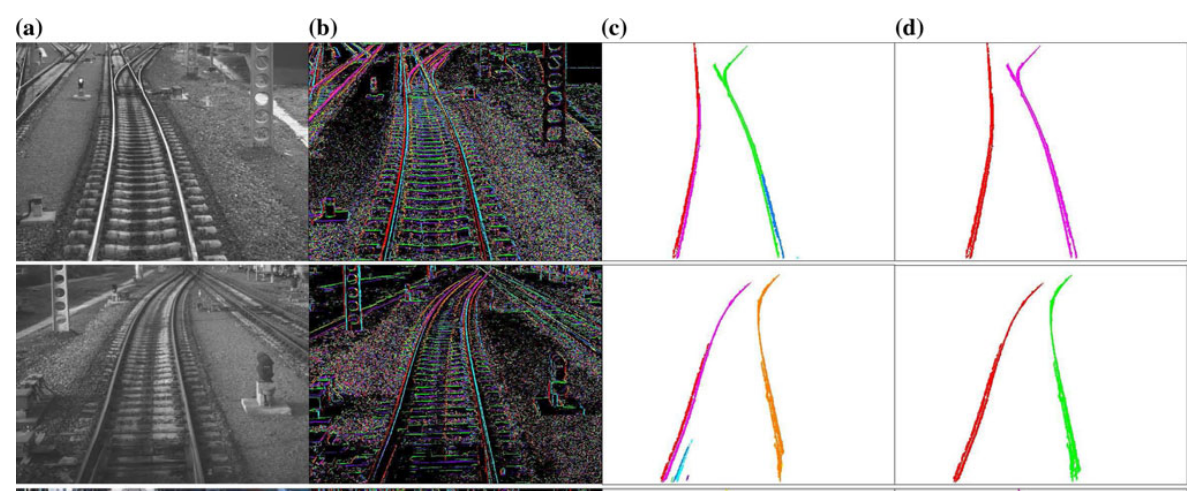
\includegraphics[width=1\linewidth]{pictures/screenshot010}
	\caption{}
	\label{fig:screenshot010}
\end{figure}

\newpage
\subsection{Поиск объекта по ключевым точкам}
Одним из методов поиска объектов на изображении является построение SIFT\cite{b:SIFT} дескриптора и сопоставление этого дескриптора с SIFT дескриптором искомого объекта.

Сначала изображение преобразуется в большой набор векторов признаков(SIFT дескриптор), каждый из которых инвариантен относительно параллельного переноса изображения, масштабирования и вращения, частично инвариантен изменению освещения и устойчив к локальным геометрическим искажениям.

После чего SIFT дескриптор текущего изображения и искомого объекта сопоставляются и на выходе можно увидеть соответствие ключевых точек на изображении и ключевых точек искомого объекта:
\begin{figure}[!h]
	\centering
	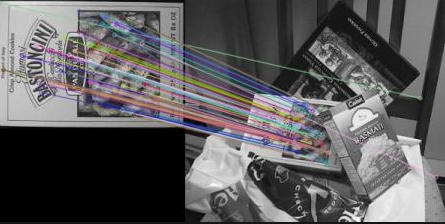
\includegraphics[width=1\linewidth]{pictures/screenshot011}
	\caption{}
	\label{fig:screenshot011}
\end{figure}

Если говорить о применении техники SIFT для поиска пересечений ж/д путей на изображении. То можно создать некоторую базы с различными видами стрелок и их SIFT дескрипторами. 

Тогда алгоритм для поиска пересечений на входном изображении будет следующий:
\begin{enumerate}
	\item Вычислять SIFT дескриптор входного изображения
	\item Сопоставить его с каждым из SIFT дескрипторов, находящихся в базе данных.
	\item Если было найдено достаточно точное сопоставление - выполнить уточнение места пересечения и добавить его в выходной результат
\end{enumerate}

\newpage
\subsection{Обучение классификатора на размеченных данных}
Распространенным способом поиска объекта на изображении является обучение классификатора на размеченных данных.

Рассмотрим классификацию с помощью SVM(машина опорных векторов)\cite{b:SVM}.
Постановка задачи: \newline
Необходимо классифицировать данные, каждый объект которых представляется как точка $x^p$ в p-мерном пространстве. Каждая из точек пренадлежит одному из двух классов. Необходим построить гиперплоскость размерности $p-1$, которая линейно разделяла бы входные точки. 
Таких гиперплоскостей может быть много, но необходимо найти ту, расстояние до которой от любого класса был бы максимальным. Что эквивалентно тому, что сумма расстояний от крайних точек классов до плоскости максимальна. 
Если такая гиперплоскость существует, она называется оптимальной разделяющей гиперплоскостью, а соответствующий ей линейный классификатор называется оптимально разделяющим классификатором.

\newpage
На вход алгоритма подается набор пар: [($x_1, c_1$), ($x_1, c_1$), ..., ($x_n, c_n$)]

Уравнение искомой гиперплоскости плоскости имеет вид:
$wx - b = 0$, где w - перпендикуляр к разделяющей плоскости, а b - расстояние от плоскости до начала координат.\newline
$wx - b = 1$ и $wx - b = -1$, соответствуют плоскостям, проходящим через крайние точки классов:
\begin{figure}[!h]
	\centering
	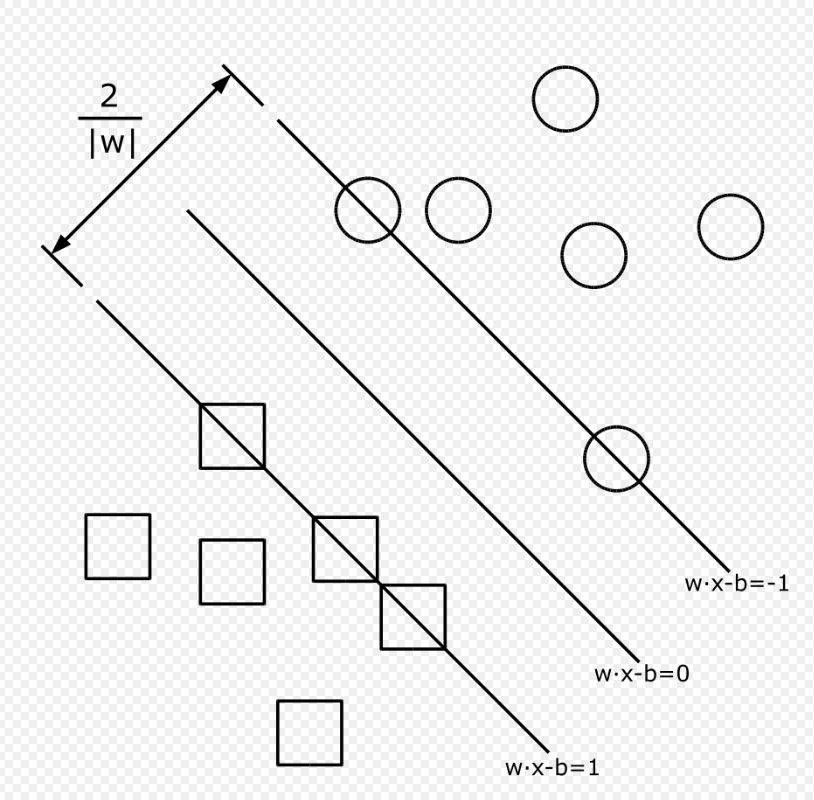
\includegraphics[width=0.5\linewidth,height=0.5\linewidth]{pictures/screenshot021}
	\caption{}
	\label{fig:screenshot021}
\end{figure}

Для полного разделения классов необходимо чтобы для всех i $\in [1, n]$ были выполнены неравенства:
\begin{equation}
\begin{cases}
wx_i - b \ge 1, c_i == 1 \\
wx_i - b \le -1, c_i == -1
\end{cases}
\label{eq:ref1}
\end{equation}

Тогда для того, чтобы найти оптимальную гиперплоскость нужно минимизировать $||w||$, при условиях \ref{eq:ref1}, что соотвествует такой задаче минимизации:
\begin{equation}
\begin{cases}
||w||^2 -> \min \\
c_i(wx_i - b) \ge 1, i \in [1, n]
\end{cases}
\label{eq:ref2}
\end{equation}

В случае, если классы не разделимы линейно, вводится дополнительный параметр $\epsilon_i \ge 0$, характеризующий ошибку на объектах $x_i$. Таким образом, смягчим ограничение во втором уравнении системы \ref{eq:ref2} и введём штраф за ошибку C - данный параметр позволяет регулировать соотношение между максимизацией ширины разделяющей полосы и минимизацией ошибки:
\begin{equation}
\begin{cases}
\dfrac{1}{2}||w||^2 + C\sum_{i=1}^{n}\epsilon_i -> \min_{wb\epsilon_i} \\
c_i(wx_i - b) \ge 1 - \epsilon_i, i \in [1, n] \\
\epsilon_i \ge 0
\end{cases}
\label{eq:ref3}
\end{equation}

Теперь, понимая математический аппарат работы SVM рассмотрим процесс построения классификатора для поиска объекта на изображении.

Входными векторами для SVM могут выступать различные виды признаков искомого объекта. Например, гистограмма ориентированных градиентов(HOG)\cite{b:HOG}, SIFT\cite{b:SIFT}/SURF\cite{b:SURF} дескрипторы.
Таким образом для решения задачи поиска объекта с помощью SVM необходимо выполнить следующие шаги:
\begin{enumerate}
	\item Разметить некоторое количество искомых объектов на изображении. Такие объекты будем относить к первому классу.
	\item Сгенерировать(или разметить) некоторое количество отрицательных примеров, которые точно не являются искомым объектом. Такие объекты отнесем ко второму классу.
	\item Рассчитать вектор признаков по которым мы будем обучать классификатор в каждой из размеченных(сгенерированных) точках изображения.
	\item Построить разделяющую объекты разных классов гиперплоскость, используя посчитанные в предыдущем пункте вектора признаков объектов.
	\item Для нахождения объекта на входном изображении, используя технику "скользящее окно"\cite{b:window} рассчитать вектор признаков во всевозможных окнах и определить по какую сторону от гиперплоскости находится вычисленный вектор. 
	Таким образом в итоге получится некоторый набор окон, в которых был найден искомый объект:
	\begin{figure}[h!]
		\centering
		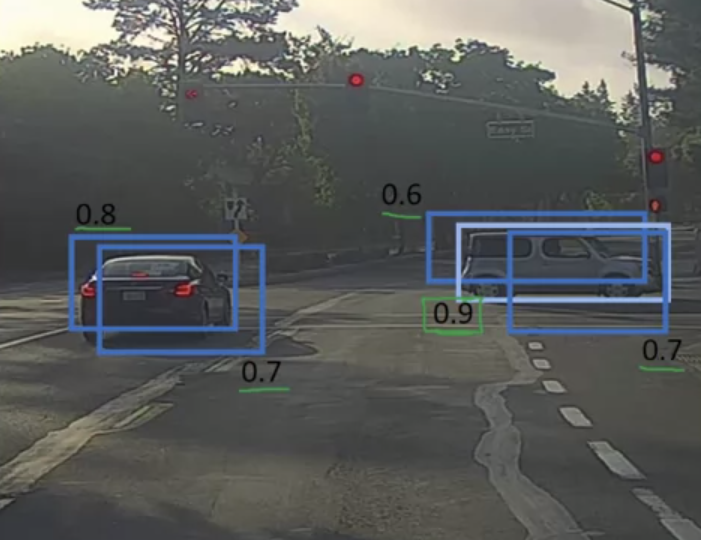
\includegraphics[width=0.7\linewidth]{pictures/screenshot024}
		\caption{}
		\label{fig:screenshot024}
	\end{figure}
	\newpage
	\item Из найденных окон выбрать наиболее точно описывающее искомый объект. Это можно сделать выбрав окно с максимальной вероятностью нахождения искомого объекта. Например, на рисунке \ref{fig:screenshot024} для правой машины это будет окно с вероятностью 0,9.
\end{enumerate}

\chapter{Основная часть}
\section{Метод, основанный на преобразовании Хафа}
\subsection{Преобразование Хафа}
\label{hough}
Преобразование Хафа \cite{b:hough_transform} - алгоритм для поиска геометрических объектов на изображении(линии, круги и т.д). В нашем случае понадобится алгоритм Хафа для поиска прямых линий на изображении. 

На вход алгоритму подается набор точек, на выходе имеется набор прямых в координатах $(\rho, \theta)$, где $\rho$ - расстояние от начала координат до прямой, $\theta$ - угол между перпендикуляром к прямой, проведенным из начала координат, и осью абсцисс.
\newline
Алгоритм:
\newline
Имеется массив аккумулятор A[M, N], где M - квантованные значения параметра $\rho$, N - квантованные значения параметра $\theta$. Изначально в каждой ячейке A находится значения ноль.
\newline
Через каждую входную точку проводятся прямые с различными параметрами $\theta$ $\in$ [0, $\pi$]. \ref{fig:hough1}

\begin{figure}[h!]
	\centering
	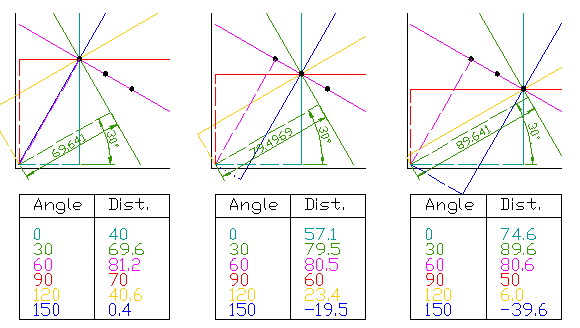
\includegraphics[width=0.7\linewidth]{pictures/hough1}
	\caption[Алгоритм Хафа]{}
	\label{fig:hough1}
\end{figure}

Каждая прямая голосует за свои параметры ($\rho$, $\theta$), то есть значение значения аккумулятора A[$\rho$, $\theta$] увеличивается на единицу. 
После голосования максимумы в массиве аккумуляторе соответствуют параметрам итоговых прямых. 

\subsection{Алгоритм метода}
\subsection{Поиск границ на изображении}
Первым шагом метода является поиск границ на входном изображении. Это делается с помощью алгоритма Canny \cite{b:canny}. Алгоритм состоит из пяти важных шагов:
\begin{enumerate}
	\item Сглаживание изображения для удаления шумов. Это делается фильтрацией изображения с использованием фильтра Гаусса: \newline
	$G(x, y, \sigma) = \dfrac{1}{2\pi\sigma^2}\exp^{\dfrac{-(x^2 + y^2)}{2\sigma^2}}$
	\item Поиск градиентов. Границы выделяются там, где находятся максимумы градиентов. Градиенты ищутся с помощью оператора Собеля, который является аналогом производной в дискретном пространстве. 
	Псевдокод поиска градиентов с помощью оператора Собеля:
	\begin{figure}[!h]
		\centering
		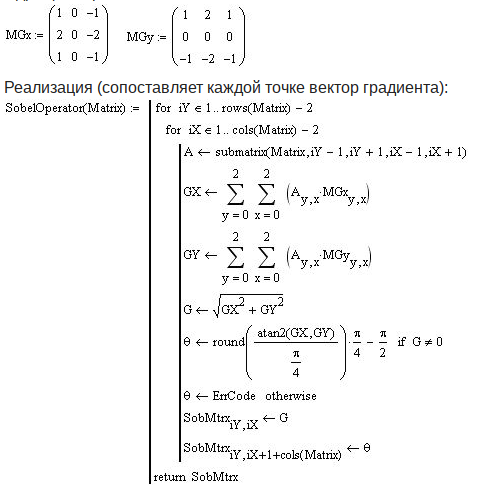
\includegraphics{pictures/sobel}
		\caption[Поиск градиентов]{}
		\label{fig:sobel}
	\end{figure}
	\item Подавление не-максимумов. Среди всех максимумов оставляем только те, что являются локальными максимумами в окрестности.
	\item Двойная пороговая фильтрация. Если значения градиента в точке максимума ниже порога - эта точка отсекается. Таким образом, чем выше значение порога, тем меньше границ будет найдено на изображении. Фильтрация в алгоритме Canny является двойной, лучше всего этот момент разъясняет иллюстрация \ref{fig:cannyth}, здесь только зелёные точки будут выбраны граничными.
	\begin{figure}[!h]
		\centering
		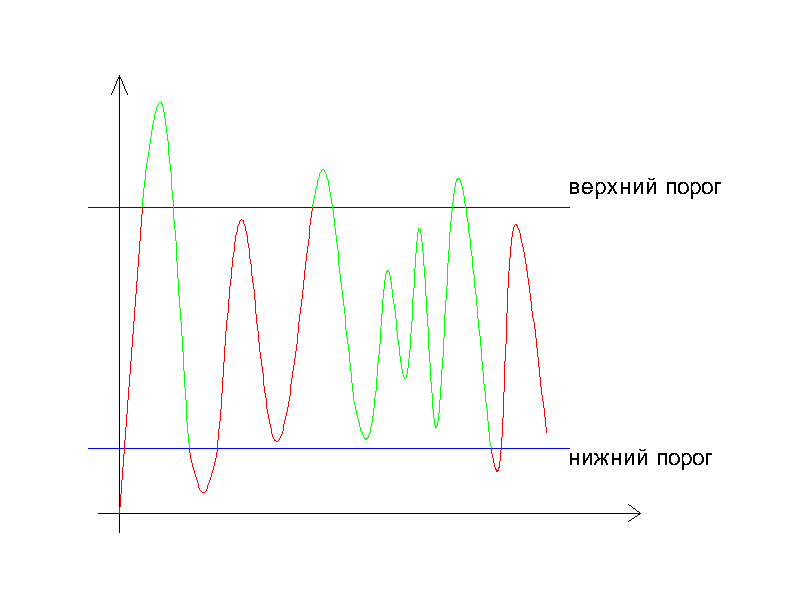
\includegraphics[width=0.7\linewidth]{pictures/canny_th}
		\caption[Двойная фильтрация]{}
		\label{fig:cannyth}
	\end{figure}
	В нашем случае значение верхнего порога вычисляется с помощью бинаризации Отцу\cite{b:otsu}. Значение нижнего порога берется как половина от значения верхнего порога. За счёт такого выбора порога достигается нормальное выявление границ на изображения с различным уровнем освещенности.
	\newpage
	\item Трассировка области неоднозначности. Итоговые границы определяются путём удаления всех краёв, несвязанных с "сильными" границами. Проще говоря, пиксели, которые не относятся ни к какой группе - подавляются.
\end{enumerate}
Пример применения алгоритма Canny к входному изображению:
\begin{figure}[!h]
	\centering
	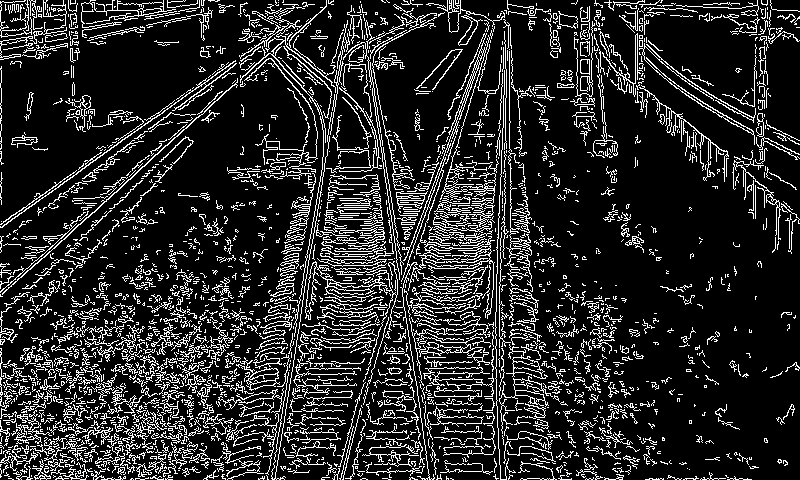
\includegraphics[width=0.9\textwidth]{pictures/canny_res}
	\caption[Применение алгоритма Canny]{}
	\label{fig:cannyres}
\end{figure}

\subsection{Разбиение изображения на горизонтальные блоки}
Сначала разбиваем изображение на горизонтальные блоки \ref{fig:horizontal_blocks}. Размер блоков уменьшается в зависимости от координаты Y на изображении, это сделано для учета перспективной проекции объектов из реального мира на изображении - чем дальше объект, тем меньше он на изображении.
\newline
Формула для расчёта размера блока в зависимости от координаты y:
\newline
$blockSize = minBlockSize + \dfrac{maxBlockSize - minBlockSize}{imageHeight - maxBlockSize}y$, где  minBlockSize = 7pix, maxBlockSize = 45pix. Данные значения были выбраны из соображений минимизации процента ошибочных предсказаний стрелок и максимизации процента предсказания реальных стрелок.
В идеале размер горизонтального блока нужно рассчитывать с использованием правил перспективного проецирования\cite{b:projection}, но для этого необходимо знать параметры камеры(угол наклона, расстояния до земли).
В нашем случае эти параметры не известны, поэтому blockSize рассчитывается просто с помощью линейной интерполяции в зависимости от координаты Y.

\begin{figure}[!h]
	\centering
	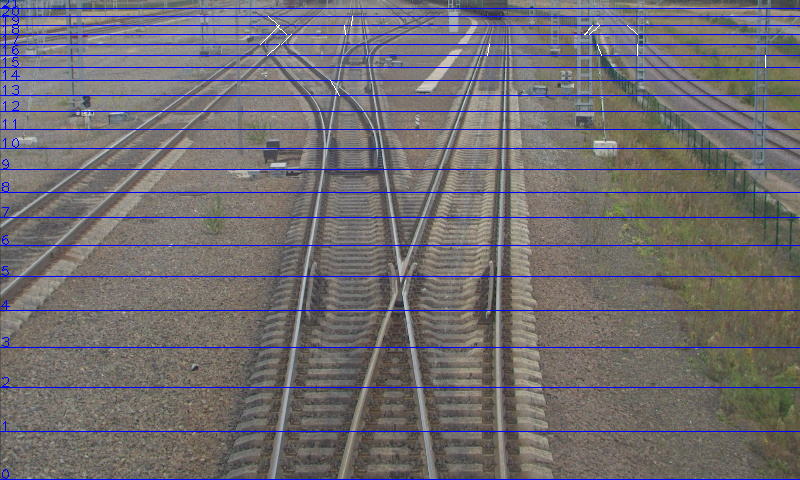
\includegraphics[width=0.9\textwidth]{pictures/horizontal_blocks.png}
	\caption[Разбиение на горизонтальные блоки]{}
	\label{fig:horizontal_blocks}
\end{figure}
\newpage
\subsection{Поиск рельсов}\label{rails_find}
Теперь рассмотрим процесс поиска рельсов на изображении, полученном после применения алгоритма Canny\ref{fig:cannyres}.

После разбиения \ref{fig:horizontal_blocks} в каждом из горизонтальных блоков ищутся прямые линии с помощью алгоритма Хафа \cite{b:hough_transform}. Можно заметить, что прямые близкие к горизонтальным можно отсекать, т.к. они не могут относиться к рельсам. Таким образом, будем искать прямые с помощью модифицированной алгоритма Хафа, в котором $\theta \in [0;\dfrac{\pi}{3}] \cup [\dfrac{2\pi}{3};\pi]$. В качестве порогового значения аккумулятора будем использовать: $\dfrac{2\cdot blockSize}{3}$, это нужно для отсечения маленьких прямых.

Результат применения алгоритма(красным выделены найденные прямые линии в каждом блоке):
\begin{figure}[!h]
	\centering
	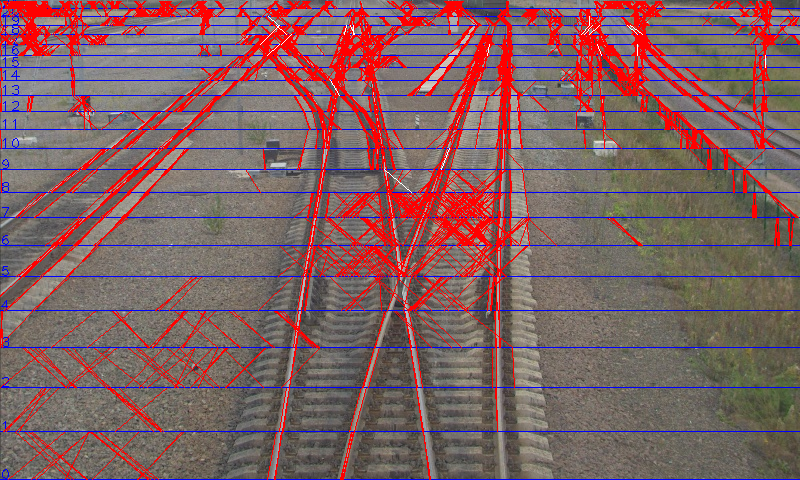
\includegraphics[width=0.9\textwidth]{pictures/hough_lines_res}
	\caption[Результат применения алгоритма]{}
	\label{fig:houghlinesres}
\end{figure}

\newpage
Можно заметить много прямых образованных на шпалах(между рельсами). Это связано с тем, что на шпалах находится много граничных точек\ref{fig:cannyres}. 
Чтобы минимизировать влияние таких прямых произведем простое удаление горизонтальных рёбер: из изображения, полученного с помощью преобразования Canny удалим такие горизонтальные участки, на которых ребро встречается 3 и более пикселей подряд.
В результате получим такую картинку ребер на изображении:
\begin{figure}[!h]
	\centering
	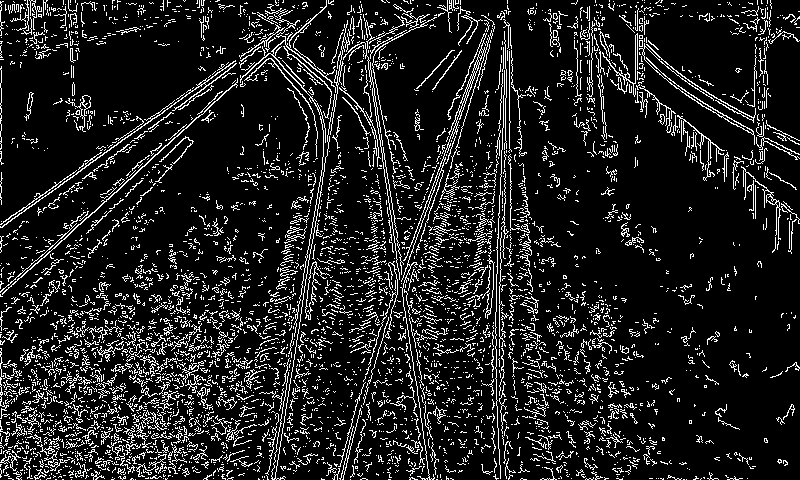
\includegraphics[width=0.9\linewidth]{pictures/screenshot0014}
	\caption{}
	\label{fig:canny_remove_horizontal}
\end{figure}

Также видно, что от одного рельса может появляться сразу несколько прямых. Чтобы этого избежать применим аппроксимацию близких прямых одной средней прямой(координаты такой прямой будут считаться, как центр масс всех близких прямых). 
Прямые будут считаться близкими, если расстояние между верхними и нижними точками соответствующих прямых меньше заданного: \newline
$LinesEps = minLinesEps + \dfrac{maxLinesEps - minLinesEps}{imageHeight - maxLinesEps}y$, \newline 
где minLinesEps = 10 и maxLinesEps = 20 - значения полученные с учетом подсчета средней ширины рельса на изображении в зависимости от координаты Y.

Тогда после описанных выше преобразований получим следующий результат:
\begin{figure}[!h]
	\centering
	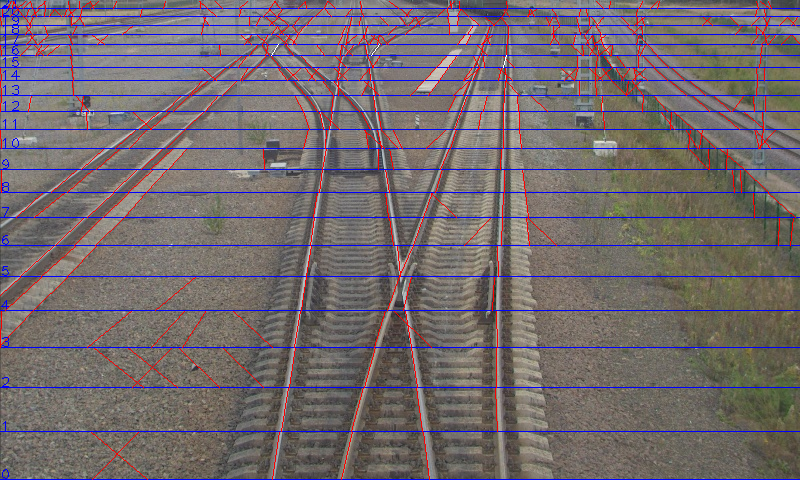
\includegraphics[width=0.9\linewidth]{pictures/screenshot0013}
	\caption{}
	\label{fig:screenshot0013}
\end{figure}

\subsection{Поиск стрелок}
\paragraph{Построение графа прямых}
\label{line_graph}

Построим граф, вершинами которого будут найденные прямые. Каждая вершина будет иметь структуру: 

$(p1, p2, high_neighs, low_neighs)$, где $p1$ - нижняя точка прямой, $p2$ - верхняя точка прямой, $high_neighs$ - верхние соседи(прямые, которые выходят из прямой, соответствующей текущей вершине), $low_neighs$ - нижние соседи(прямые, которые входят в прямую, соответствующую текущей вершине). 

Ребра в графе будут строиться по следующему принципу: начиная с нижнего горизонтального блока, для каждой прямой(curLine) ищем верхних соседей в следующем блоке. Прямая(nextLine) будет считать верхним соседом, если:

$|nextLine.p1.x - curLine.p2.x| < LinesEps$, 
где LinesEps - считается также как в параграфе \ref{rails_find}.

Найденные вершины добавляются, как верхние соседи, в текущую вершину. А также текущая вершина добавляется, как нижний сосед, в каждого из верхних соседей.

Например, на рисунке \ref{fig:neighscheck}:
\begin{enumerate}
	\item прямые 1, 2 являются верхними соседями для прямой 4. А прямая 4 является нижним соседом для прямых 1 и 2.
	\item Прямая 3 лежит дальше, чем blockEps от прямой 4, поэтому между ними нет связи в графе.
	\item прямая 4 является верхним соседом для прямых 5 и 6, но не является верхним соседом для прямой 7. А прямые 5 и 6 в свою очередь являются нижними соседями для прямой 4.
\end{enumerate}
\begin{figure}[!h]
	\centering
	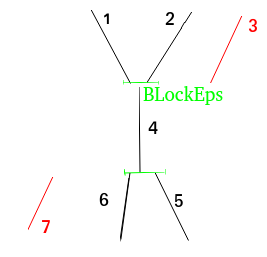
\includegraphics[width=0.7\textwidth]{pictures/neighs_check}
	\caption[Создание ребер]{}
	\label{fig:neighscheck}
\end{figure}

\paragraph{Поиск стрелок в графе}

В этом параграфе будет рассмотрен алгоритм поиска стрелок в построенном на предыдущем шаге графе. 

Алгоритм поиска пересекающихся вершин в графе: \newline
В цикле для каждой вершины графа производим следующие действия:
\begin{enumerate}
	\item Если вершина не имеет параллельного нижнего соседа - переходим к следующей вершине
	\item Для каждой пары верхних соседей текущей вершины проверяем, пересекаются ли они(\ref{intersection}), если да - верхнюю точку текущей вершины добавляем в итоговый результат найденных стрелок. Таким образом, будут найдены \nameref{fig:ycross} и \nameref{fig:xcross} пересечения.
	\begin{figure}[!h]
		\centering
		\begin{minipage}{0.45\textwidth}
			\centering
			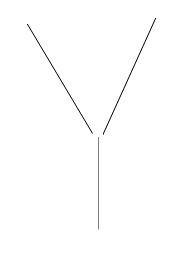
\includegraphics[width=0.7\linewidth,height=0.7\linewidth]{pictures/Y_cross}
			\caption[Y]{}
			\label{fig:ycross}
		\end{minipage}
		\begin{minipage}{0.45\textwidth}
			\centering
			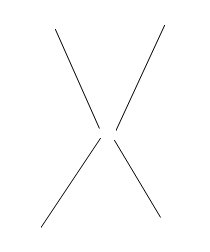
\includegraphics[width=0.7\linewidth,height=0.7\linewidth]{pictures/X_cross}
			\caption[X]{}
			\label{fig:xcross}
		\end{minipage}
	\end{figure}
	
	\item Пункт 2) повторяется для нижних соседей текущей вершины. Таким образом, будут найдены \nameref{fig:ycrossrevert} и \nameref{fig:xcross_revert} образные пересечения.
	\begin{figure}[!h]
		\centering
		\begin{minipage}{0.45\textwidth}
			\centering
			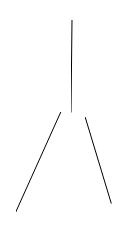
\includegraphics[width=0.7\linewidth,height=0.7\linewidth]{pictures/Y_cross_revert}
			\caption[Y - обратное]{}
			\label{fig:ycrossrevert}
		\end{minipage}
		\begin{minipage}{0.45\textwidth}
			\centering
			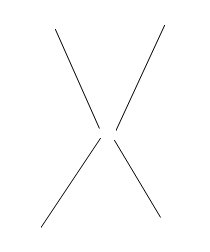
\includegraphics[width=0.7\linewidth,height=0.7\linewidth]{pictures/X_cross}
			\caption[X]{}
			\label{fig:xcross_revert}
		\end{minipage}
	\end{figure}
\end{enumerate}
\newpage

\paragraph{Алгоритм проверки параллельности прямых}
Рассмотрим функцию проверки параллельности прямых:
\begin{enumerate}
	\item Вычисляем косинусы между прямыми и осью абсцисс.
	\begin{lstlisting}
	Ox = (1, 0)
	cos1 = cos(line1, Ox)
	cos2 = cos(line2, Ox)
	\end{lstlisting}
	\item Вычисляем разность косинусов
	\begin{lstlisting}
	cos_diff = abs(cos1, cos2)
	\end{lstlisting}
	\item Вычисляем насколько близко должны быть прямые, чтобы считать их параллельными. Тут в очередной раз применяется линейная интерполяция. Так как чем ближе рельсы к камере, тем меньше угол должен быть между ними, чтобы посчитать их параллельными. Параметры max\_parallel\_cos и min\_paralle\_cos были получены экспериментально, рассматривая результаты работы алгоритма для крайних случаев 
	реальных параллельных прямых на разных уровнях высоты.
	\begin{lstlisting}
	max_parallel_cos = 0.4
	min_paralle_cos = 0.05
	parallel_cos_eps = max_parallel_cos - (max_parallel_cos - 
	min_paralle_cos) / image_height * current_y
	\end{lstlisting}
	\item Если разность косинусов, вычисленная ранее, меньше parallel\_cos\_eps, прямые считаются параллельными.
	\begin{lstlisting}
	return cos_diff < parallel_cos_eps
	\end{lstlisting}
\end{enumerate}              
\paragraph{Алгоритм проверки пересечения вершин}
\label{intersection}
На вход поступают v1, v2 -вершины, для которых нужно определить пересекаются ли они.
А также параметры: глубина проверки пересечений(intersection\_depth) и глубина проверки соседей(check\_neighs\_depth).
\newline
Алгоритм:
\begin{enumerate}
	\item Если глубина проверки пересечений достигла 0 - возвращаем True - вершины пересекаются.
	\begin{lstlisting}
	if intersection_depth == 0:
	return True
	\end{lstlisting}
	\item Если прямые, соответствующие вершинам НЕ параллельны - выбираем у каждой прямой параллельного верхнего соседа. Если параллельные соседи существуют, рекурсивно вызываем функцию is\_intersection с уменьшенной на единицу глубиной поиска пересечений.
	\begin{lstlisting}
	if not is_parallel(v1, v2):
	parallel_1 = v1.getParallelNeigh()
	parallel_2 = v2.getParallelNeigh()
	if parallel_1 and parallel_2:
	return is_intersection(parallel_1, parallel_2,
	intersection_depth - 1, check_neighs_depth)
	\end{lstlisting}
	\item Если глубина проверки соседей ещё не достигла нуля И у текущих вершин v1, v2 существуют параллельные им верхние соседи, то рекурсивно вызываем is\_intersection для найденных параллельных верхних соседей с уменьшенной на единицу глубиной проверки соседей.
	\begin{lstlisting}
	if check_neighs_depth > 0:
	parallel_1 = v1.getParallelNeigh()
	parallel_2 = v2.getParallelNeigh()
	if parallel_1 and parallel_2:
	return is_intersection(parallel_1, parallel_2,
	intersection_depth, check_neighs_depth - 1)
	\end{lstlisting}
	\item Если не было выполнено ни одно из первых трех условий - вершины не являются пересекающимися - вернем False.
\end{enumerate}
Описанный выше алгоритм применяется как для проверки пересечения между верхними соседями, так и между нижними соседями. 

Рассмотрим алгоритм на примере(синими линями изображены границы горизонтальных блоков): 
\newline
В данном примере рассматривается прямая 1. \newline На вход функции is\_intersection поступают соседние прямые 2 и 3, и параметры intersection\_depth = 2, check\_neighs\_depth = 1.
\newline
Если прямые 2 и 3 НЕ параллельны, то запускаем is\_intersection для прямых 4 и 5 и intersection\_depth = 1, check\_neighs\_depth = 1.
\newline
Если прямые 4 и 5 НЕ параллельны, то запускаем  is\_intersection для прямых 6 и 7 и intersection\_depth = 0, check\_neighs\_depth = 1. Теперь функция возвращает True и верхняя точка прямой 1 добавляется, как стрелка в результат.
\begin{figure}[!h]
	\centering
	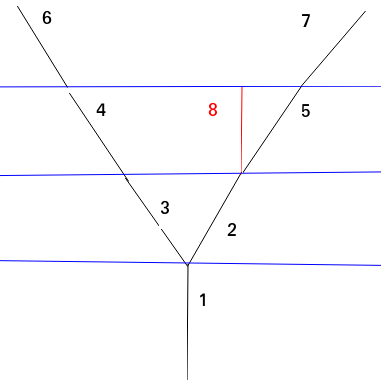
\includegraphics[width=0.7\linewidth]{pictures/intersection_example}
	\caption[Intersection]{}
	\label{fig:intersectionexample}
\end{figure}

В случае пересечений между нижними соседями пример будет зеркально отражен по оси Y.

\newpage
Параметр check\_neighs\_depth нужен в случае, когда сами соседи являются параллельными(прямые 2 и 3), но их продолжения(прямые 4 и 5) уже НЕ являются параллельными. Такая ситуация характерна для Y пересечений, которые находятся близко к камере.
\begin{figure}[!h]
	\centering
	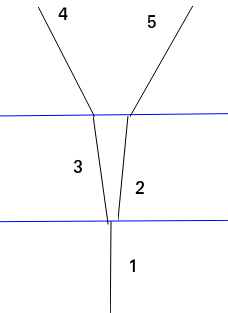
\includegraphics[width=0.5\textwidth, height=0.4\textheight]{pictures/intersection_example1}
	\caption{}
	\label{fig:intersectionexample1}
\end{figure}
\paragraph{Аппроксимация близких вершин}
На последнем этапе близкие по расстоянию стрелки аппроксимируются их центрами масс.
Эта процедура повторяется рекурсивно, пока в результирующем массиве все стрелки не станут полностью отделимыми друг от друга.

\newpage			
\subsection{Описание данных для тестирования}
Для тестирования алгоритма было размечено 204 фотографии ж/д путей, сделанных с локомотива. Часть фотографий была сделана при дневном свете \ref{fig:res1}, а часть при искусственном \ref{fig:res3}. Также имеются изображения, сделанные в летний\ref{fig:res1} и в зимний период \ref{fig:res4}.
\paragraph{Параметры датасета}
\begin{enumerate}
	\item Всего стрелок размечено: 1308
	\item Среднее количество стрелок на одном изображении: 6.3
	\item Около 70\% изображений сделаны в летний период. Около 30\% в зимний.
\end{enumerate}


\newpage
\subsection{Результаты}
\paragraph{Примеры работы алгоритма}
Рассмотрим результаты работы алгоритма на различных изображениях.
\newline
Результаты работы на изображении сделанном при дневном:
\begin{figure}[!h]
	\centering
	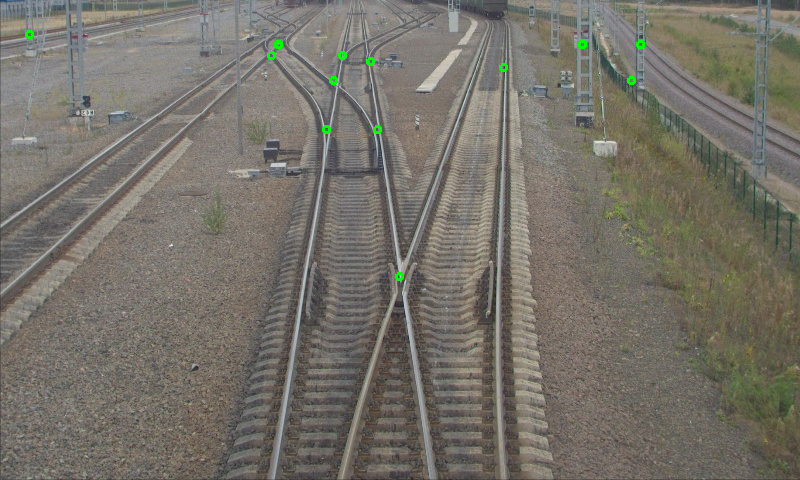
\includegraphics[width=0.7\linewidth]{pictures/screenshot0015}
	\caption{}
	\label{fig:res1}
\end{figure}
\begin{figure}[!h]
	\centering
	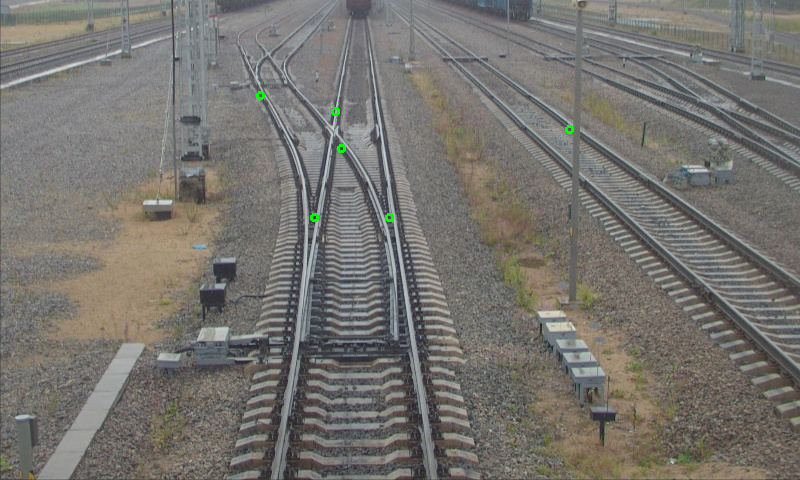
\includegraphics[width=0.7\linewidth]{pictures/screenshot0016}
	\caption{}
	\label{fig:res2}
\end{figure}
\newpage

Истинное положение стрелок (маркеры) на рисунках \ref{fig:res1}, \ref{fig:res2}, \ref{fig:res3}, \ref{fig:res4} - не обозначены, так как их положения очевидны

Видно, что есть большие стрелки - те, которые находятся достаточно близко к камере, алгоритм распознает очень хорошо. С маленькими стрелками есть небольшие проблемы, например на изображении \ref{fig:res2} самая дальняя маленькая стрелка слева не распозналась.\newline
Также видно, что достаточно много false positive стрелок получившихся от столбов и заборов. Один из способов их подавления - использовать алгоритм Region growing up(\cite{b:growing_up}) для сегментации изображения снизу вверх.

Теперь рассмотрим результат работы алгоритма при других погодных условиях и искусственном свете. Видно, что алгоритм хорошо справляется и с такими изображениями.
\begin{figure}[!h]
	\centering
	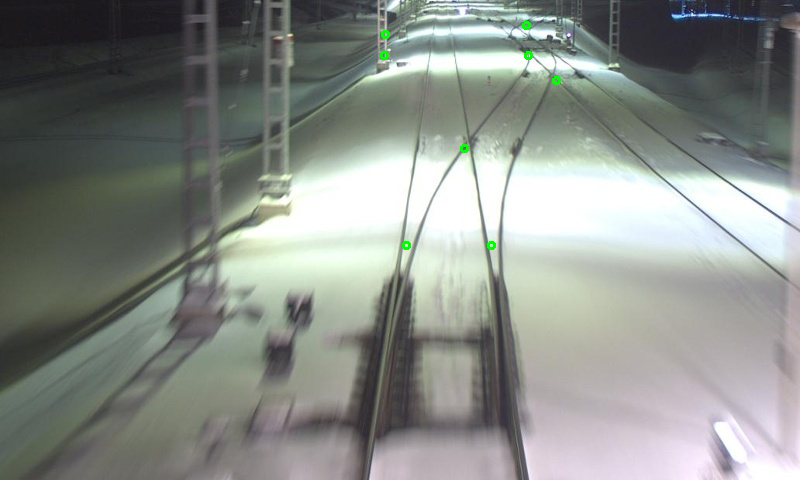
\includegraphics[width=0.7\linewidth]{pictures/screenshot0017}
	\caption{}
	\label{fig:res3}
\end{figure}

\newpage
Теперь посмотрим на пример изображения, на котором алгоритм выдал очень плохой результат:
\begin{figure}[h!]
	\centering
	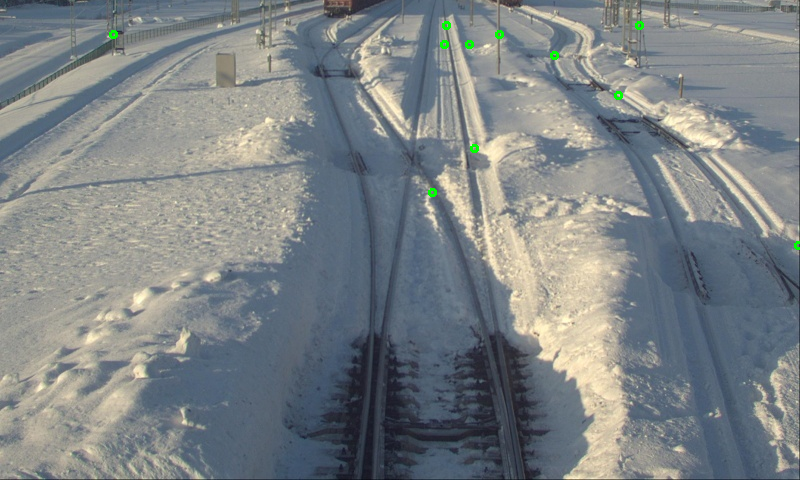
\includegraphics[width=0.7\linewidth]{pictures/screenshot0018}
	\caption{}
	\label{fig:res4}
\end{figure}
Видно, что на изображении есть ярко освещенные солнцем участки, и темная тень от поезда, в связи с этим алгоритм Отцу \cite{b:otsu} выдал достаточно высокое значение пороговых фильтров и рельсы, находящиеся в тени не были восприняты как рёбра алгоритмом Canny\cite{b:canny}. В следствии чего соответствующие рельсам линии не были найдены алгоритмом Хафа \cite{b:hough_transform}.
\begin{figure}[h!]
	\centering
	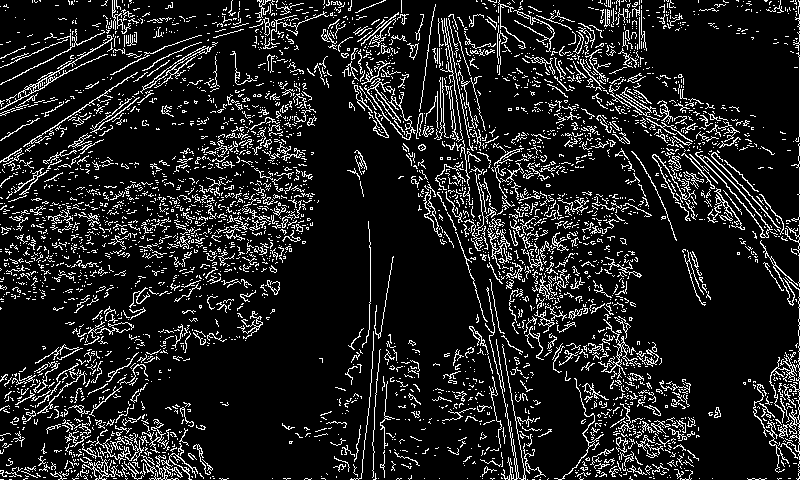
\includegraphics[width=0.7\linewidth]{pictures/screenshot0019}
	\caption{}
	\label{fig:bad_canny}
\end{figure}
\begin{figure}[h!]
	\centering
	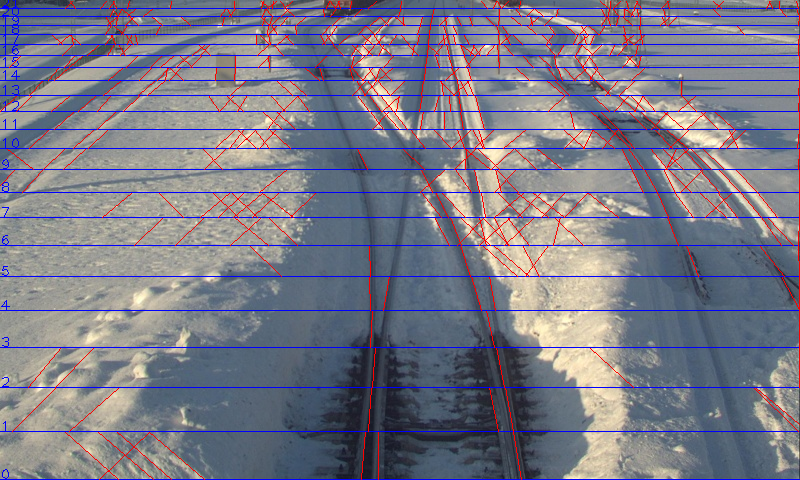
\includegraphics[width=0.7\linewidth]{pictures/screenshot0020}
	\caption{}
	\label{fig:bad_lines}
\end{figure}

\newpage
\paragraph{Статистические результаты}
Вспомним о том, что мы не знаем параметры камеры и поэтому ширину горизонтальных блоков выбираем с помощью линейной интерполяции \ref{line_graph}. Интерполяция происходит между значениями maxBlockSize и minBlockSize. 
Рассмотрим зависимость результатов обнаружения от выбора этих параметров:
\begin{table}[!h]
	\begin{tabular}{|c|c|c|l|l|}
		\hline
		\multicolumn{1}{|l|}{\textbf{minBlockEps}} & \multicolumn{1}{l|}{\textbf{maxBlockEps}} & \multicolumn{1}{l|}{\textbf{time(s)}} & \textbf{Precision} & \textbf{Recall} \\ \hline
		7                                          & 45                                        & 0.8                                   & 0.27               & 0.92            \\ \hline
		7                                          & 30                                        & 5.5                                   & 0.22                & 0.97            \\ \hline
		20                                         & 45                                        & 0.08                                  & 0.4               & 0.44             \\ \hline
	\end{tabular}
\end{table}
\newline
$Precistion = \dfrac{TruePositive}{TruePositive + FalsePositive}$ - процент корректных предсказаний.
\newline
$Recall = \dfrac{TruePositive}{TruePositive + FalseNegative}$ - мера, определяющая как хорошо алгоритм находит позитивные примеры(стрелки)

\newpage
Видно, что при уменьшении максимального размера блока растёт время работы алгоритма. Уменьшается процент корректных предсказаний. И увеличивается количество найденных положительных примеров. 

Также и в обратную сторону, если увеличивать минимальный размер блока, то время работы уменьшается, НО количество найденных положительных примеров и процент корректных предсказаний уменьшаются. 

При большой нижней границе minBlockEps далекие стрелки вообще не находятся, зато хорошо ищутся близкие стрелки, вот пример для minBlockEps = 20pix:
\begin{figure}[!h]
	\centering
	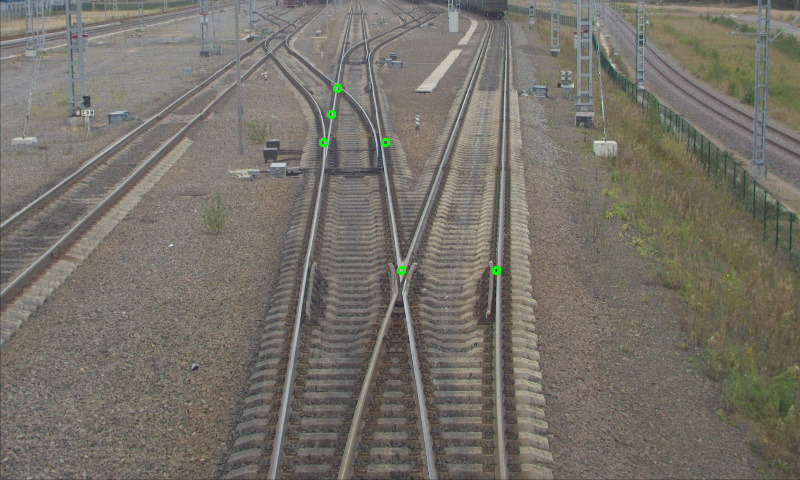
\includegraphics[width=0.7\linewidth]{pictures/45_20.png}
	\caption[Y - обратное]{}
	\label{fig:45_20}
\end{figure}


\newpage
\addcontentsline{toc}{section}{Список литературы}
\begin{thebibliography}{2}
	\bibitem{b:hough_transform}
	\textbf{Преобразование Хафа}. Википедия. [Электронный ресурс] URL - 
	\href{https://en.wikipedia.org/wiki/Hough\_transform}{https://en.wikipedia.org/wiki/Hough\_transform}
	
	\bibitem{b:canny}
	\textbf{Алгоритм Canny}. [Электронный ресурс] URL - 
	\href{https://habr.com/ru/post/114589/}{https://habr.com/ru/post/114589/}
	
	\bibitem{b:otsu}
	\textbf{Алгоритм Отцу}. [Электронный ресурс] URL - 
	\href{https://docs.opencv.org/2.4/doc/tutorials/imgproc/threshold/threshold.html}{https://docs.opencv.org/2.4/doc/tutorials/imgproc/threshold/threshold.html}
	
	\bibitem{b:projection}
	\textbf{Перспективная проекция}. [Электронный ресурс] URL - 
	\href{http://stratum.ac.ru/education/textbooks/kgrafic/lection04.html}{http://stratum.ac.ru/education/textbooks/kgrafic/lection04.html}
	
	\bibitem{b:growing_up}
	\textbf{Efficient railway tracks detection and turnouts recognition method using HOG features}. [Электронный ресурс] URL - 
	\href{https://link.springer.com/article/10.1007/s00521-012-0846-0}{https://link.springer.com/article/10.1007/s00521-012-0846-0}
	
	\bibitem{b:hough_work1}
	\textbf{Vision based rail track and switch recognition for self-localization of trains in a rail network}. [Электронный ресурс] URL - 
	\href{https://ieeexplore.ieee.org/document/5940466?denied=}{https://ieeexplore.ieee.org/document/5940466?denied=}
	
	\bibitem{b:HOG}
	\textbf{Histogram of oriented gradients}. Википедия. [Электронный ресурс] URL - 
	\href{https://en.wikipedia.org/wiki/Histogram_of_oriented_gradients}{https://en.wikipedia.org/wiki/Histogram\_of\_oriented\_gradients}
	
	\bibitem{b:SIFT}
	\textbf{Scale-invariant feature transform}. [Электронный ресурс] URL - 
	\href{https://en.wikipedia.org/wiki/Scale-invariant_feature_transform}{https://en.wikipedia.org/wiki/Scale-invariant\_feature\_transform}
	
	\bibitem{b:edge_match}
	\textbf{Using Partial Edge Contour Matches for Efficient Object Category
		Localization ,Hayko Riemenschneider, Michael Donoser and Horst
		BischofProceedings of European Conference on Computer Vision}. [Электронный ресурс] URL - 
	\href{http://www.icg.tugraz.at/Members/hayko/partial-contour-efficient-
		matching}{http://www.icg.tugraz.at/Members/hayko/partial-contour-efficient-
		matching}
	
	\bibitem{b:SURF}
	\textbf{Speeded up robust features}. [Электронный ресурс] URL - 
	\href{https://en.wikipedia.org/wiki/Speeded\_up_robust\_features}{https://en.wikipedia.org/wiki/Speeded\_up\_robust\_features}
	
	\bibitem{b:SVM}
	\textbf{Support Vector Machine}. [Электронный ресурс] URL - 
	\href{https://en.wikipedia.org/wiki/Support\_vector\_machine}{https://en.wikipedia.org/wiki/Support\_vector\_machine}
	
	\bibitem{b:decision_tree}
	\textbf{Decision tree}. [Электронный ресурс] URL - 
	\href{https://en.wikipedia.org/wiki/Decision\_tree}{https://en.wikipedia.org/wiki/Decision\_tree}
	
	\bibitem{b:knn}
	\textbf{K-nearest neighbors algorithm}. [Электронный ресурс] URL - 
	\href{https://en.wikipedia.org/wiki/K-nearest\_neighbors\_algorithm}{https://en.wikipedia.org/wiki/K-nearest\_neighbors\_algorithm}
	
	\bibitem{b:window}
	\textbf{Sliding window}. [Электронный ресурс] URL - 
	\href{https://www.pyimagesearch.com/2015/03/23/sliding-windows-for-object-detection-with-python-and-opencv/}{https://www.pyimagesearch.com/2015/03/23/sliding-windows-for-object-detection-with-python-and-opencv/}
	
\end{thebibliography}		  		 		